\section{Case study}
In order to focus on the implementation of the hybrid machine learning algorithm, a CPS, with ready to use datasets, was chosen from a list provided in \cite{morris_industrial_nodate}: the \textbf{power system} \cite{adhikari_power_2014}, which network diagram was represented on figure \ref{fig:cps_rep}. The system is composed of two power generators who are alimenting the whole system. Intelligent Electronic Devices (IEDs) R1 to R4 and the breakers BR1 to BR4 can be found connected directly to those generators. Each IED switches its corresponding breaker when a fault is detected, valid or fake. The communication between the IEDs and the Substation Switch is done wirelessly. On the other hand the Substation Switch is connected with the Primary Domain Controller (PDC) and the Control Room.

\begin{figure}[H]
    \centering
    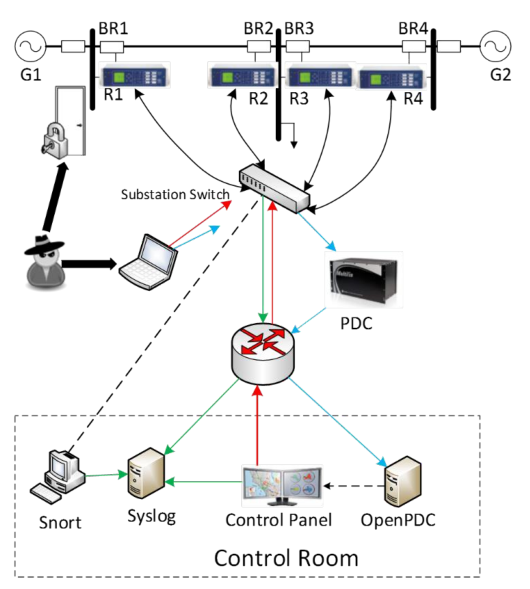
\includegraphics[width=100mm]{images/cps_rep.png}
    \caption[Power system network diagram]{Power system network diagram \cite{adhikari_power_2014}}
    \label{fig:cps_rep}
\end{figure}

The operation of this power system can be described following 6 main scenarios:
\begin{itemize}
    \item normal behaviour, 
    \item short-circuit,
    \item line maintenance,
    \item remotely opening the breakers (attack),
    \item disruption of fault protection system (attack),
    \item fault imitation (attack).
\end{itemize} 
Each of those scenarios can be divided into several sub-scenarios concerning different entities of the system or/and the failure range. Every scenario was labelled with a number between 1 and 41. In this way \textbf{37 scenarios} are obtained, divided and numbered as follows:
\begin{itemize}
    \item 1 no events scenario, its number it is 41,
    \item 8 natural fault scenarios, its number ranges are 1-6 (short-circuit) and 13-14 (line maintenance),
    \item 28 attack scenarios, its number ranges are 7-12 (fault imitation), 15-20 (remotely opening the breakers), 20-30 and 35-40 (disruption of fault protection system).
\end{itemize}
The reason for dropping the numbers between 31 and 34 in the naming process of scenarios is not known.

The datasets provided in \cite{morris_industrial_nodate} represent \textbf{78377 events}, in which one of those scenarios was reproduced in the system. They have been grouped by scenario into 3 datasets: binary (attack or normal operation), three-class (attack, normal fault and no events) and multiclass (differentiating all 37 scenarios). Each of these 3 datasets is composed of 15 .arff or .csv files comporting in average 141 events for each of 37 scenarios. The exact number of events per file for each scheme is illustrated on figure \ref{fig:scen_distro_37}. For the 3 class dataset \textbf{55663 attack}, \textbf{18309 natural fault} and \textbf{4405 normal operation} events were found. The distribution of these schemes throughout the files is shown on figure~\ref{fig:scen_distro_file}. 

\begin{figure}[H]
    \centering
    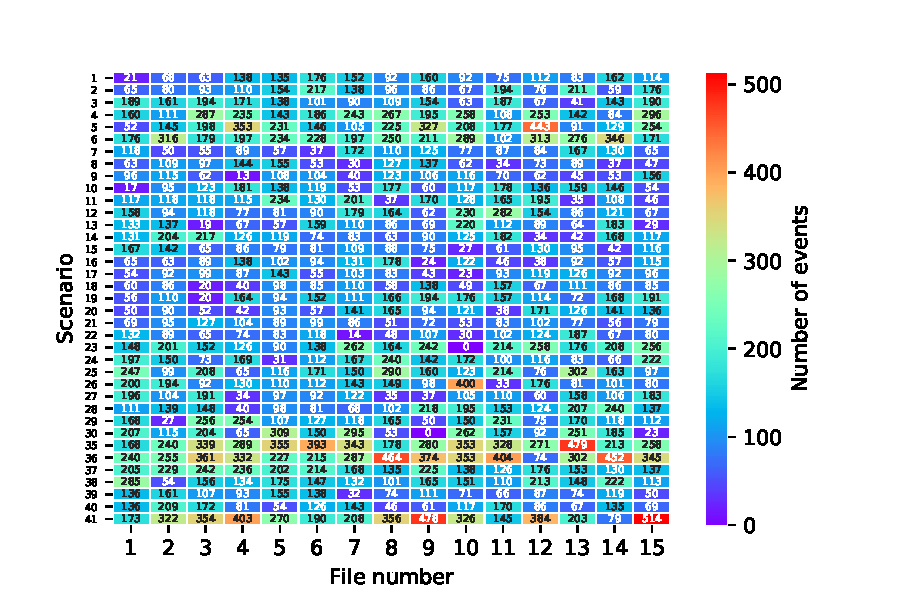
\includegraphics[]{images/distr_allscen.pdf}
    \caption{Scenarios distribution throughout all 15 files} \label{fig:scen_distro_37}
\end{figure}

\begin{figure}[H]
    \centering
    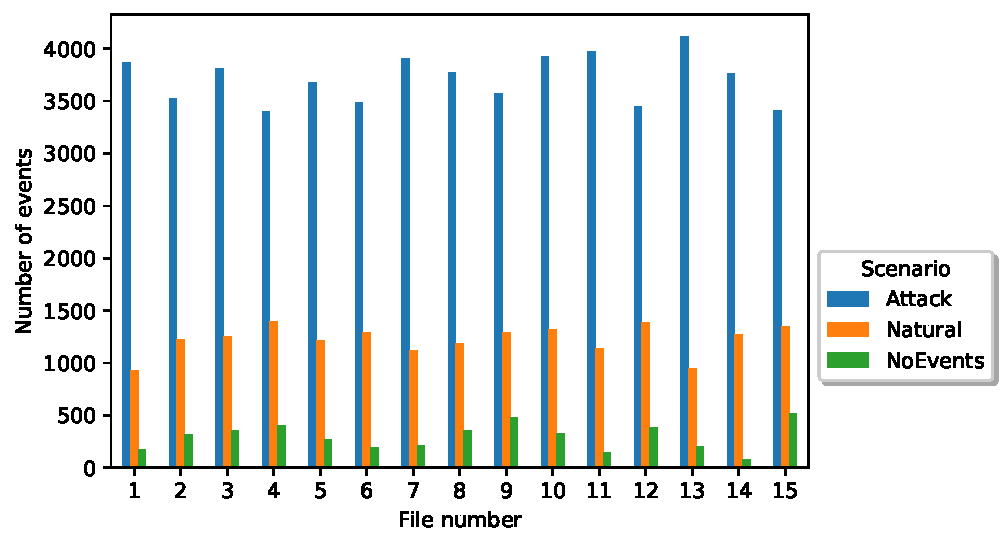
\includegraphics[]{images/distr_3classes.pdf}
    \caption{Scenarios distribution throughout the 3-class dataset files}
    \label{fig:scen_distro_file}
\end{figure}

Figure \ref{fig:scen_distro_file} shows also this distribution for the binary datasets, it is sufficient to add the number of natural (orange) and normal operation (green) events.

The scenarios are not equally distributed in the case of the 37 schemes dataset, it is especially shown by the standard deviation of 61, which is an important value compared to some scenarios counting less than 100 events. On the other hand, in the case of 3-class scenarios, the distribution is even more not equal compared to the 37 schemes dataset. The \textbf{mean standard deviation among all files is equal to 1767}, which is an enormous result given that some scenarios count only around 100 events.

Each of previously mentioned events is described by \textbf{128 features}: 116 provided by four phasor measurement units\footnote{Phasor measurement units measure the electrical waves on an electricity grid} (each one provides 29 types of measurements) and 12 other features are reserved for control panel logs, snort alerts, relay logs of 4 phasors. The mentioned 116 features, each has a label formed by \textbf{concatenation} of the \textbf{source phasor reference} (it can be R1, R2, R3, R4) and the \textbf{measurement name}, as provided in table \ref{tab:pmu_mes}. For example R4-PM5:I stands for phase B current phase magnitude measured by R4.
%give exemple - preciser plus les features 
%expliquer les features plus
%figure pour explication de phase, magnitude

\begin{table}[H]
    \centering
    \caption[Phasor measurements]{Phasor measurements \cite{adhikari_power_2014}} \label{tab:pmu_mes}
    \begin{tabular}{lr}
        \toprule
        Feature&Description \\
        \midrule
        PA1:VH – PA3:VH&Phase A-C Voltage Phase Angle \\
        PM1:V – PM3:V&Phase A-C Voltage Phase Magnitude \\
        PA4:IH – PA6:IH&Phase A-C Current Phase Angle \\
        PM4:I – PM6:I&Phase A-C Current Phase Magnitude \\
        PA7:VH – PA9:VH&Pos.–Neg.– Zero Voltage Phase Angle \\
        PM7:V – PM9:V&Pos.–Neg.–Zero Voltage Phase Magnitude \\
        PA10:VH - PA12:VH&Pos.–Neg.–Zero Current Phase Angle \\
        PM10:V - PM12:V&Pos.–Neg.–Zero Current Phase Magnitude \\
        F&Frequency for relays \\
        DF&Frequency Delta (dF/dt) for relays \\
        PA:Z&Appearance Impedance for relays \\
        PA:ZH&Appearance Impedance Angle for relays \\
        S&Status Flag for relays \\
        \bottomrule
    \end{tabular}
\end{table} 

Those datasets have been used in several works related to CPS cyber-attack classification, one of which is \cite{borges_hink_machine_2014-1}, where the author try to find the most accurate algorithm to predict the status of the power system. The following chapter shows an attempt to partially reproduce the results obtained by them.
